% [原文 p.59]
\begin{corollary*}{2.5.4}
  映射 $[H]\mapsto t$ 给出同构 $K(P(\C^n))\cong\Z[t]/(t-1)^n$。
\end{corollary*}

\begin{proof}
  取 $X$ 为一点即可。
\end{proof}

与前面相同，命题 2.5.3 中的有限群也可以作用；此时得到
\[
K_G(X)[t]\Big/\prod_{i=1}^{n}\bigl(t-[L_i^*]\bigr)\;\cong\;K_G\bigl(P(L_1\oplus\cdots\oplus L_n)\bigr).
\]

\section{$K^*(X,Y)$ 中的乘法}
\takeaway{本节用外部积把相对 K 群的乘法按次数拼接，核心工具是复合形范畴 $C_n(X,A)$：欧拉示性数把复合形的同伦类与 $K(X,A)$ 等同，于是乘法化归为复形的张量积，外积代数又给出 Thom 类。}

首先注意，$K(X)$ 的乘法可以用下面的“外部积”来定义。设 $E,F$ 为 $X$ 上的向量丛，令 $E\hat\otimes F$ 为 $X\times X$ 上的向量丛 $\pi_1^*(E)\otimes\pi_2^*(F)$。设 $\Delta\colon X\to X\times X$ 为对角映射，则 $E\otimes F=\Delta^*(E\hat\otimes F)$。

% [Tutor Note: 原书用 $\hat\otimes$ 表示外部张量积、用 $\otimes$ 表示普通张量积：$E\hat\otimes F$ 定义在积空间 $X\times Y$ 上，而 $E\otimes F$ 只在同一底空间上才有意义，它是 $\Delta^*$ 的拉回。初读时容易把两者混为一谈。]
设 $E$ 为 $X$ 上的向量丛，$F$ 为 $Y$ 上的向量丛，则 $X\times Y$ 上的向量丛 $E\hat\otimes F=\pi_X^*(E)\otimes\pi_Y^*(F)$ 由此确定，它定义了积
\[
K(X)\otimes K(Y)\longrightarrow K(X\times Y).
\]
当 $X,Y$ 带基点时，$\tilde K(X\wedge Y)$ 是 $\tilde K(X\times Y)\to\tilde K(X)\oplus\tilde K(Y)$ 的核，因此得到 $\tilde K(X)\otimes\tilde K(Y)\to\tilde K(X\wedge Y)$。

若 $(X,A),(Y,B)$ 为空间对，则得到
\[
\tilde K(X/A)\otimes\tilde K(Y/B)\longrightarrow\tilde K\bigl((X/A)\wedge(Y/B)\bigr),
\]
亦即
\[
K(X,A)\otimes K(Y,B)\longrightarrow K\bigl(X\times Y,\;(X\times B)\cup(A\times Y)\bigr).
\]
我们就把 $(X,A)\times(Y,B)$ 定义为 $\bigl(X\times Y,(X\times B)\cup(A\times Y)\bigr)$。

当 $X=Y$ 时，有对角映射 $\Delta\colon(X,A\cup B)\to(X,A)\times(X,B)$，它给出 $K(X,A)\otimes K(X,B)\to K(X,A\cup B)$。特别地，取 $B=\varnothing$ 可知 $K(X,A)$ 是 $K(X)$ 模。

% [原文 p.60]
进一步，
\[
K(X,A)\longrightarrow K(X)\longrightarrow K(A)
\]
是 $K(X)$ 模的完全序列，这也容易看出。

更一般地，对 $m,n\ge 0$ 如下定义积
\[
K^{-n}(X,A)\otimes K^{-m}(Y,B)\longrightarrow K^{-n-m}\bigl((X,A)\times(Y,B)\bigr).
\]
由于
\begin{align*}
K^{-n}(X,A)&=\tilde K\bigl(S^n\wedge(X/A)\bigr),\\
K^{-m}(Y,B)&=\tilde K\bigl(S^m\wedge(Y/B)\bigr),
\end{align*}
可得
\begin{align*}
K^{-n}(X,A)\otimes K^{-m}(Y,B)&\longrightarrow\tilde K\bigl(S^n\wedge(X/A)\wedge S^m\wedge(Y/B)\bigr)\\
&=\tilde K\bigl(S^n\wedge S^m\wedge(X/A)\wedge(Y/B)\bigr)\\
&=K^{-n-m}\bigl((X,A)\times(Y,B)\bigr).
\end{align*}
因此，取对角映射 $\Delta\colon(X,A\cup B)\to(X,A)\times(X,B)$，对 $x\in K^{-n}(X,A)$、$y\in K^{-m}(X,B)$，用 $\Delta^*(x\otimes y)$ 定义积 $xy\in K^{-n-m}(X,A\cup B)$。此时由引理 2.4.11 知 $xy=(-1)^{mn}yx$。

令
\[
K^{\#}(X,A)=\sum_{n=0}^{\infty}K^{-n}(X,A).
\]
此时 $K^{\#}(X)$ 是分次环，$K^{\#}(X,A)$ 是分次 $K(X)$ 模。设 $\beta\in K^{-2}(*)$ 为生成元，则乘 $\beta$ 对一切 $n$ 诱导同构 $K^{-n}(X,A)\to K^{-n-2}(X,A)$。令 $K^*(X,A)=K^{\#}(X,A)/(1-\beta)$，则 $K^*(X)$ 是 $\Z/2$ 分次环，$K^*(X,A)$ 是 $K^*(X)$ 上的 $\Z/2$ 分次模。

% [Tutor Note: 这里的 $\beta$ 就是 Bott 元素。乘 $\beta$ 给出的平移同构 $K^{-n}\cong K^{-n-2}$ 正是 Bott 周期性的实质内容；而 $K^*=K^{\#}/(1-\beta)$ 把这条周期性直接做成环的商，故 $K^*$ 只在模 2 意义下分次。]
对任意对 $(X,A)$，完全序列的三角形
\[
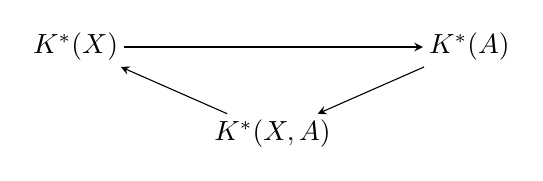
\begin{tikzpicture}[baseline=(current bounding box.center),>=stealth,
  every node/.style={inner sep=2pt}]
\node (X)  at (0,1.1)  {$K^*(X)$};
\node (A)  at (5,1.1)  {$K^*(A)$};
\node (XA) at (2.5,0)  {$K^*(X,A)$};
\draw[->] (X)  -- (A);
\draw[->] (XA) -- (X);
\draw[->] (A)  -- (XA);
\end{tikzpicture}
\]
中的每个映射都是 $K^*(X)$ 模的映射。其证明只有边界算子 $\delta$ 的情形较难，故作为引理 2.6.1 先行给出。

% [原文 p.61]
\begin{lemma*}{2.6.1}
  $\delta\colon K^{-1}(Y)\to K^0(X,Y)$ 是 $K(X)$ 模同态。
\end{lemma*}

\begin{proof}
  按定义，$\delta$ 由空间对的包含映射
  \[
  j\colon\bigl(X\times\{1\}\cup Y\times I,\;Y\times\{0\}\bigr)\longrightarrow
  \bigl(X\times\{1\}\cup Y\times I,\;Y\times\{0\}\cup X\times\{1\}\bigr)
  \]
  诱导（参见下图）。
  \[
  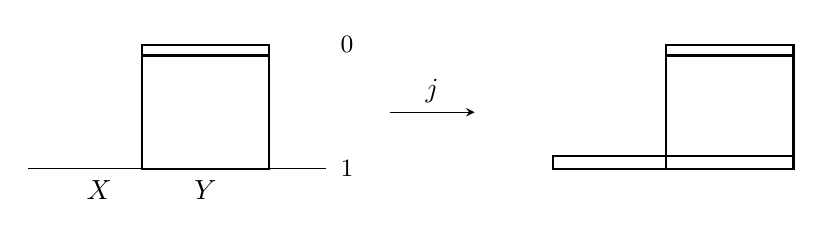
\begin{tikzpicture}[baseline=(current bounding box.center),>=stealth,scale=0.9]
    % 左图：X×{1} ∪ Y×I，粗带为 Y×{0}
    \draw (0,0) -- (4.2,0);
    \draw[thick] (1.6,0) rectangle (3.4,1.6);
    \draw[thick] (1.6,1.6) rectangle (3.4,1.75);
    \draw (0,0) -- (4.2,0);
    \node at (4.5,1.75) {\small $0$};
    \node at (4.5,0) {\small $1$};
    \node at (1.0,-0.3) {$X$};
    \node at (2.5,-0.3) {$Y$};
    % 中间的 j
    \draw[->] (5.1,0.8) -- (6.3,0.8) node[midway,above] {$j$};
    % 右图：粗带为 Y×{0} 与 X×{1}
    \begin{scope}[xshift=7.4cm]
      \draw[thick] (0,0) rectangle (3.4,0.18);
      \draw[thick] (1.6,0) rectangle (3.4,1.6);
      \draw[thick] (1.6,1.6) rectangle (3.4,1.75);
      \draw (0,0) -- (3.4,0);
    \end{scope}
  \end{tikzpicture}
  \]
  于是 $\delta=j^*$ 是群 $K(X\times\{1\}\cup Y\times I)\cong K(X)$ 上的模同态。剩下只需说明 $K^{-1}(Y)$ 与 $K^0(X,Y)$ 的 $K(X)$ 模结构都是标准的。$K^{-1}(Y)$ 的情形一目了然。至于 $K^0(X,Y)$，只要注意到投影 $I\to\{1\}$ 诱导同构映射
  \begin{gather*}
  K^0(X,Y)\to K\bigl(X\times\{1\}\cup Y\times I,\;Y\times\{0\}\bigr),\\
  K(X)\to K\bigl(X\times\{1\}\cup Y\times I\bigr)
  \end{gather*}
  即可。
\end{proof}

这里暂且离开正题，给出 $K(X,A)$ 的另一种描述。这种描述尤其与积结构相容。

对 $n\ge 1$，如下定义范畴 $C_n(X,A)$。$C_n(X,A)$ 的对象是 $X$ 上的向量丛 $E_n,E_{n-1},\dots,E_0$ 连同映射 $\alpha_i\colon E_i|_A\to E_{i-1}|_A$，

% [原文 p.62]
使得
\[
0\longrightarrow E_n|_A\xrightarrow{\ \alpha_n\ }E_{n-1}|_A\xrightarrow{\ \alpha_{n-1}\ }\cdots\xrightarrow{\ \alpha_1\ }E_0|_A\longrightarrow 0
\]
成为完全序列者。设 $E=(E_i,\alpha_i)$，$F=(F_i,\beta_i)$，则射 $\varphi\colon E\to F$ 由映射 $\varphi_i\colon E_i\to F_i$（$i=0,\dots,n$）组成，并满足 $\beta_i\varphi_i=\varphi_{i-1}\alpha_i$。特别地，$C_1(X,A)$ 由 $X$ 上的向量丛 $E_1,E_0$ 与同构映射 $\alpha\colon E_1|_A\cong E_0|_A$ 组成。

$C_n(X,A)$ 的基本列是指 $E_p=E_{p-1}$ 且 $\alpha_p$ 为恒等映射的序列
\[
0\longrightarrow\cdots\longrightarrow 0\longrightarrow E_p|_A\xrightarrow{\ \cong\ }E_{p-1}|_A\longrightarrow 0\longrightarrow\cdots\longrightarrow 0.
\]
等价关系 $E\sim F$ 定义为：存在基本列 $Q_1,\dots,Q_n,P_1,\dots,P_m$ 使
\[
E\oplus Q_1\oplus\cdots\oplus Q_n\cong F\oplus P_1\oplus\cdots\oplus P_m.
\]
按这个等价关系分出的等价类之集记作 $\mathcal{L}_n(X,A)$。显然，对每个 $n$，$\mathcal{L}_n(X,A)$ 是半群。

有自然的包含映射 $C_n(X,A)\subset C_{n+1}(X,A)$，它诱导同态 $\mathcal{L}_n(X,A)\to\mathcal{L}_{n+1}(X,A)$。$C_n(X,A)$ 全体之和集记作 $C_\infty(X,A)$，$\mathcal{L}_n(X,A)$ 的归纳极限记作 $\mathcal{L}_\infty(X,A)$。

本节的主定理是下面的定理 2.6.2。

\begin{theorem*}{2.6.2}
  对一切 $n\ge 1$，映射 $\mathcal{L}_n(X,A)\to\mathcal{L}_{n+1}(X,A)$ 是同构，且 $\mathcal{L}_n(X,A)\cong K(X,A)$。
\end{theorem*}

这个定理的证明分解为若干引理。

先考虑 $A=\varnothing$，$n=1$ 的特殊情形。此时 $C_1(X,\varnothing)$ 由所有的向量丛对 $(E_1,E_0)$ 组成。$(E_1,E_0)\sim(F_1,F_0)$ 当且仅当存在向量丛 $Q,P$ 使 $E_1\oplus Q\cong F_1\oplus P$，$E_0\oplus Q\cong F_0\oplus P$。此时映射 $\mathcal{L}_1(X,\varnothing)\to K(X)$ 由 $(E_1,E_0)\mapsto[E_0]-[E_1]$ 给出，并且是同构。事实上，$\mathcal{L}_1(X,\varnothing)$ 与 2.1 节所述的 $K(X)$ 的定义之一一致。

% [原文 p.63]
\begin{definition}{2.6.3}
  $\mathcal{L}_n$ 的欧拉示性数 $\chi_n$ 是指函子的自然变换
  \[
  \chi_n\colon\mathcal{L}_n(X,A)\longrightarrow K(X,A),
  \]
  并且当 $A=\varnothing$ 时恒有 $\chi_n(E_n,E_{n-1},\dots,E_0)=\sum(-1)^i[E_i]$。
\end{definition}

% [Tutor Note: 定义 2.6.3 说的是“自然变换”，即 $\chi_n$ 对所有空间对 $(X,A)$ 同时给出，并与拉回相容；只在某个固定对上有交替和并不足以确定它。$\chi_n$ 的存在性要到引理 2.6.8 才证明。]
首先需要下面的简单引理。

\begin{lemma*}{2.6.4}
  设 $A\subset X$，$E$ 与 $F$ 为 $X$ 上的向量丛。设 $\varphi\colon E|_A\to F|_A$，$\psi\colon E\to F$ 为单射同态（或同构映射），并假设 $\psi|_A$ 与 $\varphi$ 同伦。此时 $\varphi$ 可延拓为 $X$ 上的单射同态（或同构映射）。
\end{lemma*}

\begin{proof}
  令 $Y=(A\times[0,1])\cup(X\times\{0\})$。设 $E',F'$ 分别为 $E,F$ 在投影 $Y\to X$ 下的拉回；此时存在单射同态（或同构映射）$\Phi\colon E'\to F'$，满足 $\Phi|_{A\times\{1\}}=\varphi$ 且 $\Phi|_{X\times\{0\}}=\psi$。$\Phi$ 可延拓到 $A$ 的某个邻域 $U$ 上的 $(U\times[0,1])\cup(X\times\{0\})$。取 $f\colon X\to[0,1]$ 使 $f(A)=1$，$f(X\setminus U)=0$。此时对 $X$ 的每点 $x$，令 $\varphi_x=\Phi_{(x,f(x))}$，则 $\varphi$ 延拓到 $X$ 上。
\end{proof}

\begin{lemma*}{2.6.5}
  若 $A$ 为一点，则
  \[
  0\longrightarrow\mathcal{L}_1(X,A)\longrightarrow\mathcal{L}_1(X)\longrightarrow\mathcal{L}_1(A)
  \]
  完全。因此，设 $\chi_1$ 为 $\mathcal{L}_1$ 的欧拉示性数，若 $A$ 为一点，则 $\chi_1\colon\mathcal{L}_1(X,A)\to K(X,A)$ 是同构。
\end{lemma*}

\begin{proof}
  设 $(E_1,E_0)$ 为 $\mathcal{L}_1(X)$ 元素的代表元；若它在 $\mathcal{L}_1(A)$ 中的像为零，则 $E_1$ 与 $E_0$ 在 $A$ 上的维数相同，即存在同构 $\varphi\colon E_1|_A\to E_0|_A$。因此 $\mathcal{L}_1(X,A)\to\mathcal{L}_1(X)\to\mathcal{L}_1(A)$ 完全。

  若 $(E_1,E_0,\varphi)$ 在 $\mathcal{L}_1(X)$ 中的像为零，则存在平凡丛 $P$ 与同构 $\psi\colon E_1\oplus P\cong E_0\oplus P$。$\psi(\varphi\oplus1)^{-1}$ 是 $(E_0\oplus P)|_A$ 的自同构映射，
  % [原文 p.64]
  而 $A$ 为一点，故这样的自同构映射都与恒等映射同伦。因此由引理 2.6.4，它可以延拓为同构 $\alpha\colon E_0\oplus P\to E_0\oplus P$。这样便得到交换图
  \[
  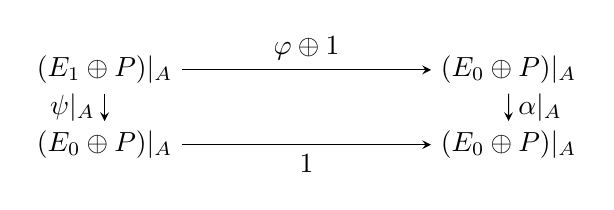
\begin{tikzpicture}[baseline=(current bounding box.center),>=stealth,scale=0.95]
  \node (TL) at (0,1)  {$(E_1\oplus P)|_A$};
  \node (TR) at (5.4,1) {$(E_0\oplus P)|_A$};
  \node (BL) at (0,0)  {$(E_0\oplus P)|_A$};
  \node (BR) at (5.4,0) {$(E_0\oplus P)|_A$};
  \draw[->] (TL) -- node[above] {$\varphi\oplus1$} (TR);
  \draw[->] (TL) -- node[left] {$\psi|_A$} (BL);
  \draw[->] (TR) -- node[right] {$\alpha|_A$} (BR);
  \draw[->] (BL) -- node[below] {$1$} (BR);
  \end{tikzpicture}
  \]
  亦即，$(E_1,E_0,\varphi)$ 是 $\mathcal{L}_1(X,A)$ 中 $0$ 的代表元。因此 $\mathcal{L}_1(X,A)\to\mathcal{L}_1(X)$ 是单射。
\end{proof}

\begin{lemma*}{2.6.6}
  对一切 $(X,A)$，$\mathcal{L}_1(X/A,A/A)\to\mathcal{L}_1(X,A)$ 是同构。因此，设 $\chi_1$ 为欧拉示性数，则对一切 $(X,A)$，$\chi_1\colon\mathcal{L}_1(X,A)\to K(X,A)$ 是同构。
\end{lemma*}

\begin{proof}
  同构 $\mathcal{L}_1(X/A,A/A)\to K(X,A)$ 经过 $\mathcal{L}_1(X,A)$ 分解，故映射 $\mathcal{L}_1(X/A,A/A)\to\mathcal{L}_1(X,A)$ 是单射。

  设 $E_1,E_0$ 为 $X$ 上的向量丛，$\alpha\colon E_1|_A\to E_0|_A$ 为同构映射。设 $P$ 为 $X$ 上的向量丛，且存在与平凡丛 $F$ 的同构 $\beta\colon E_1\oplus P\to F$。此时令 $\gamma=(\alpha\oplus1)\beta^{-1}$，则 $(E_1,E_0,\alpha)$ 与 $(F,E_0\oplus P,\gamma)$ 等价。而 $(F,E_0\oplus P,\gamma)$ 是 $(F,(E_0\oplus P)/\gamma,\gamma/\gamma)$ 的像。因此 $\mathcal{L}_1(X/A,A/A)\to\mathcal{L}_1(X,A)$ 是满射。
\end{proof}

\begin{lemma*}{2.6.7}
  若 $\chi_1,\chi_1'$ 都是 $\mathcal{L}_1$ 的欧拉示性数，则 $\chi_1=\chi_1'$。
\end{lemma*}

\begin{proof}
  $\chi_1'\chi_1^{-1}$ 是函子 $K$ 到自身的自然变换，且在各个 $K(X)$ 上是恒等映射。由于 $K(X,A)=\tilde K(X/A)$ 单射地映入 $K(X/A)$，故 $\chi_1'\chi_1^{-1}$ 对一切 $K(X,A)$ 都是恒等映射。
\end{proof}

\begin{lemma*}{2.6.8}
  $\mathcal{L}_1$ 的欧拉示性数 $\chi_1$ 存在。
\end{lemma*}

\begin{proof}
  设 $(E_1,E_0,\alpha)$ 为 $\mathcal{L}_1(X,A)$ 元素的代表元。取 $X_0,X_1$ 为 $X$ 的两个副本，令 $Y=X_0\cup_A X_1$ 为把两份 $X$ 中对应的 $A$ 的点等同起来
  % [原文 p.65]
  所得的空间。此时 $[E_1,\alpha,E_0]\in K(Y)$。设 $\pi_i\colon Y\to X_i$ 为自然收缩。此时 $K(Y)=K(Y,X_i)\oplus K(X_i)$。映射 $(X_0,A)\to(Y,X_1)$ 诱导同构映射 $K(Y,X_1)\to K(X_0,A)$。把分解 $K(Y)=K(Y,X_1)\oplus K(X_1)$ 与同构 $K(Y,X_1)\to K(X,A)$ 复合，再将 $[E_1,\alpha,E_0]$ 的像记为 $\chi_1(E_1,E_0,\alpha)\in K(X,A)$。若 $A=\varnothing$，则 $\chi_1(E_1,E_0,\alpha)=[E_0]-[E_1]$。这个定义不依赖代表元的选取，此事容易验证。
\end{proof}

\begin{corollary*}{2.6.9}
  $\mathcal{L}_1(X,A)$ 中 $(E_1,E_0,\alpha)$ 的等价类只依赖于 $\alpha$ 的同伦类。
\end{corollary*}

\begin{proof}
  令 $Y=X\times[0,1]$，$B=A\times[0,1]$。此时，若取满足 $\alpha_0=\alpha$ 的同伦 $\alpha_t$，则 $\alpha_t$ 确定同构 $\beta\colon\pi^*(E_1)|_B\cong\pi^*(E_0)|_B$。设 $i_j\colon(X,A)\to(X\times\{j\},A\times\{j\})$（$j=0,1$）。考察交换图
  \[
  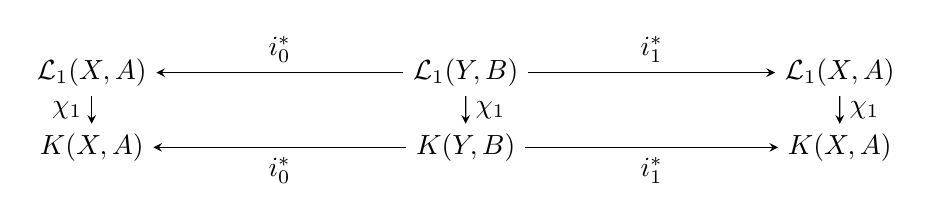
\begin{tikzpicture}[baseline=(current bounding box.center),>=stealth,scale=0.95]
  \node (TL) at (0,1)   {$\mathcal{L}_1(X,A)$};
  \node (TM) at (5,1)   {$\mathcal{L}_1(Y,B)$};
  \node (TR) at (10,1)  {$\mathcal{L}_1(X,A)$};
  \node (BL) at (0,0)   {$K(X,A)$};
  \node (BM) at (5,0)   {$K(Y,B)$};
  \node (BR) at (10,0)  {$K(X,A)$};
  \draw[->] (TM) -- node[above] {$i_0^*$} (TL);
  \draw[->] (TM) -- node[above] {$i_1^*$} (TR);
  \draw[->] (TM) -- node[right] {$\chi_1$} (BM);
  \draw[->] (TL) -- node[left] {$\chi_1$} (BL);
  \draw[->] (TR) -- node[right] {$\chi_1$} (BR);
  \draw[->] (BM) -- node[below] {$i_0^*$} (BL);
  \draw[->] (BM) -- node[below] {$i_1^*$} (BR);
  \end{tikzpicture}
  \]
  则图中映射全为同构，且 $i_0^*(i_1^*)^{-1}$ 是恒等映射，故 $[E_1,E_0,\alpha_0]=[E_1,E_0,\alpha_1]$。
\end{proof}

\begin{lemma*}{2.6.10}
  映射 $\mathcal{L}_n(X,A)\to\mathcal{L}_{n+1}(X,A)$ 对 $n\ge1$ 是满射。
\end{lemma*}

\begin{proof}
  设 $(E_{n+1},\dots,E_0;\alpha_{n+1},\dots,\alpha_1)$ 为 $\mathcal{L}_{n+1}(X,A)$ 元素的代表元，则
  \[
  (E_{n+1},\,E_n\oplus E_{n+1},\,E_{n-1}\oplus E_{n+1},\,E_{n-2},\dots,E_0;\;\alpha_{n+1},\alpha_n\oplus1,\dots,\alpha_1)
  \]
  也是 $\mathcal{L}_{n+1}(X,A)$ 元素的代表元。两个映射 $\alpha_{n+1}\oplus0\colon E_{n+1}\to E_n\oplus E_{n+1}$ 与 $0\oplus1\colon E_{n+1}\to E_n\oplus E_{n+1}$ 作为单射同态（线性地）彼此同伦。$0\oplus1$ 可延拓到 $X$，故由引理 2.6.4，$\alpha_{n+1}\oplus0$ 可延拓为 $X$ 上的单射同态 $\beta\colon E_{n+1}\to E_n\oplus E_{n+1}$。这样，$E_n\oplus E_{n+1}$ 便可写成
  % [原文 p.66]
  $\beta(E_{n+1})\oplus Q$。此时得到 $\gamma\colon Q\to E_{n-1}\oplus E_{n+1}$，并可看出 $(E_{n+1},\dots,E_0;\alpha_{n+1},\dots,\alpha_1)$ 与 $(0,Q,E_{n-1}\oplus E_{n+1},\dots,E_0;0,\gamma,\dots,\alpha_1)$ 等价。因此 $\mathcal{L}_n(X,A)\to\mathcal{L}_{n+1}(X,A)$ 是满射。
\end{proof}

\begin{lemma*}{2.6.11}
  映射 $\mathcal{L}_n(X,A)\to\mathcal{L}_{n+1}(X,A)$ 对一切 $n\ge1$ 都是同构。
\end{lemma*}

\begin{proof}
  只需构造映射 $\mathcal{L}_n(X,A)\to\mathcal{L}_1(X,A)$，使它成为 $\mathcal{L}_1(X,A)\to\mathcal{L}_n(X,A)$ 的左逆映射。

  设 $(E_n,\dots,E_0;\alpha_n,\dots,\alpha_1)$ 为 $\mathcal{L}_n(X,A)$ 元素的代表元。在每一个 $E_i$ 上选取 Hermite 度量，记 $\alpha_i^*\colon E_{i-1}|_A\to E_i|_A$ 为 $\alpha_i$ 的 Hermite 共轭。
  令 $F_0=\sum E_{2i}$，$F_1=\sum E_{2i+1}$，并用
  \[
  \beta=\sum\alpha_{2i+1}+\sum\alpha_{2i}^*
  \]
  定义 $\beta\colon F_1\to F_0$。此时 $[F_1,F_0,\beta]\in\mathcal{L}_1(X,A)$。这给出映射 $\mathcal{L}_n(X,A)\to\mathcal{L}_1(X,A)$。要说明它定义良好，只需说明它与度量的选取无关。然而度量的选法彼此同伦，故改变度量并不改变 $\beta$ 的同伦类。因此这个映射定义良好。它显然是 $\mathcal{L}_1(X,A)\to\mathcal{L}_n(X,A)$ 的左逆映射。
\end{proof}

% [Tutor Note: 引理 2.6.11 的技巧是全节的关键：把复形 $\cdots\to E_{2i}\to E_{2i-1}\to\cdots$ 的偶、奇两组直和分别记作 $F_0,F_1$，再把 $\alpha$ 与其 Hermite 共轭拼成一个映射 $\beta\colon F_1\to F_0$。由正合性，$\beta$ 是 $A$ 上的同构，于是任意长的复形都压缩为 $\mathcal{L}_1$ 中的一个元素。]
\begin{corollary*}{2.6.12}
  对每个 $n$，恰有一个欧拉示性数 $\chi_n\colon\mathcal{L}_n(X,A)\to K(X,A)$，且它总是同构。因此存在同构 $\chi\colon\mathcal{L}_\infty(X,A)\to K(X,A)$。
\end{corollary*}

下面想构造积
\[
\mathcal{L}_n(X,Y)\otimes\mathcal{L}_m(X',Y')\longrightarrow\mathcal{L}_{n+m}\bigl((X,Y)\times(X',Y')\bigr),
\]
使它成为与积
\[
K(X,Y)\otimes K(X',Y')\longrightarrow K\bigl((X,Y)\times(X',Y')\bigr)
\]
相容的积。

% [原文 p.67]
为此，必须考虑向量丛的复形，即序列
\[
0\longrightarrow E_n\xrightarrow{\ \sigma_n\ }E_{n-1}\xrightarrow{\ \sigma_{n-1}\ }\cdots\xrightarrow{\ \sigma_1\ }E_0\longrightarrow 0,
\]
且对一切 $i$ 满足 $\sigma_i\sigma_{i+1}=0$。

\begin{lemma*}{2.6.13}
  设 $E_0,\dots,E_n$ 为 $X$ 上的向量丛，$\sigma_i\colon E_i|_Y\to E_{i-1}|_Y$ 使得
  \[
  0\longrightarrow E_n\xrightarrow{\ \sigma_n\ }E_{n-1}\xrightarrow{\ \sigma_{n-1}\ }\cdots\xrightarrow{\ \sigma_1\ }E_0\longrightarrow 0
  \]
  在 $Y$ 上完全。此时对一切 $i$，存在 $\sigma_i$ 到 $X$ 的延拓 $\rho_i\colon E_i\to E_{i-1}$，并满足 $\rho_i\rho_{i+1}=0$。
\end{lemma*}

\begin{proof}
  先证：存在 $Y$ 在 $X$ 中的开邻域 $U$，以及对一切 $i$ 的 $\sigma_i$ 到 $U$ 的延拓 $\tau_i$，使得
  \[
  0\longrightarrow E_n\xrightarrow{\ \tau_n\ }E_{n-1}\xrightarrow{\ \tau_{n-1}\ }\cdots\xrightarrow{\ \tau_1\ }E_0\longrightarrow 0
  \]
  在 $U$ 上完全。于是，到整个 $X$ 的延拓可由把 $\tau_i$ 换作 $\rho\tau_i$ 得到，其中 $\rho$ 为 $X$ 上的连续函数，在 $Y$ 上 $\rho=1$，且 $\operatorname{supp}\rho\subset U$。

  设在 $Y$ 于 $X$ 中的某个闭邻域 $U_i$ 上，$\sigma_1,\dots,\sigma_i$ 已延拓为 $\tau_1,\dots,\tau_i$，且 $U_i$ 上
  \[
  E_i\xrightarrow{\ \tau_i\ }E_{i-1}\xrightarrow{\ \tau_{i-1}\ }\cdots\xrightarrow{\ \tau_1\ }E_0\longrightarrow 0
  \]
  为完全序列。设 $K_i$ 为 $\tau_i$ 在 $U_i$ 上的核。此时 $\sigma_{i+1}$ 确定 $Y$ 上 $\operatorname{Hom}(E_{i+1},K_i)$ 的一个截面。这个截面可延拓到 $U_i$ 中 $Y$ 的某邻域上，因此 $\sigma_{i+1}\colon E_{i+1}\to K_i$ 在该邻域上可延拓为 $\tau_{i+1}\colon E_{i+1}\to K_i$。由于 $\sigma_{i+1}$ 在 $Y$ 上满射，$\tau_{i+1}$ 在 $U_i$ 中 $Y$ 的某个闭邻域 $U_{i+1}$ 上也是满射。于是本引理可由对 $i$ 的归纳法得到。
\end{proof}

引入集合 $\mathcal{D}_n(X,Y)$：它是 $X$ 上长度 $n$、在 $Y$ 上非轮状（即完全）的复形之集。
% [原文 p.68]
这样的两个复形称为同伦等价的，是指它们分别同构于 $\mathcal{D}_n(X\times I,Y\times I)$ 的某个元素在 $X\times\{0\}$ 与 $X\times\{1\}$ 上的限制。自然映射
\[
\Phi\colon\mathcal{D}_n(X,Y)\longrightarrow\mathcal{L}_n(X,Y)
\]
由同态映射的限制给出。

\begin{lemma*}{2.6.14}
  $\Phi$ 诱导同伦类的双射。
\end{lemma*}

\begin{proof}
  引理 2.6.13 已证明 $\Phi$ 是满射。要证 $\Phi$ 是单射，须证明 $X\times\{0\}\cup X\times\{1\}$ 上任意在 $Y\times I$ 上非轮状的复形都能延拓为 $X\times I$ 全空间上的复形。这个延拓分如下三步进行。首先，作到 $X\times[0,1/4]$ 与 $X\times[3/4,1]$ 的平凡延拓。其次，取 $V$ 为 $Y$ 在 $X$ 中的闭邻域，使给定复形在其上仍非轮状，把引理 2.6.13 应用于 $X\times[1/4,3/4]$、$Y\times[1/4,3/4]\cup V\times\{1/4\}\cup V\times\{3/4\}$。这样便得到 $X\times[1/4,3/4]$ 上的复形，它在沿带状区域 $V\times\{1/4\}$ 与 $V\times\{3/4\}$ 加厚了的两端与已定义者一致。于是，把一切乘上满足
  \begin{enumerate}[label=(\roman*),leftmargin=2.6em,itemsep=1pt]
  \item $X\times\{0\}\cup X\times\{1\}\cup Y\times I$ 上 $\rho=1$；
  \item $(X\setminus V)\times\{1/4\}\cup(X\setminus V)\times\{3/4\}$ 上 $\rho=0$
  \end{enumerate}
  的函数 $\rho$，便得到所求的延拓（参见下图。虚线外侧表示 $\rho$ 的支集）。
  \[
  \begin{tikzpicture}[baseline=(current bounding box.center),>=stealth,scale=0.85]
    \draw[->] (0,0) -- (9.2,0) node[below] {$X$};
    \draw[->] (0,0) -- (0,4.6) node[left] {$I$};
    \draw (0,0) -- (-0.1,0) node[left] {$0$};
    \draw (0,1) -- (-0.1,1) node[left] {$\tfrac14$};
    \draw (0,3) -- (-0.1,3) node[left] {$\tfrac34$};
    \draw (0,4) -- (-0.1,4) node[left] {$1$};
    \draw[line width=2pt] (0.35,0) -- (1.05,0);
    \node at (0.7,-0.35) {\small $Y$};
    \draw (0.2,0.15) -- (0.2,0.3) -- (1.25,0.3) -- (1.25,0.15);
    \node at (0.72,0.5) {\small $V$};
    \draw (1.7,1) -- (9,1);
    \draw (1.7,3) -- (9,3);
    \draw[dashed] (1.7,4.4) -- (1.7,0.75) -- (9,0.75);
  \end{tikzpicture}
  \]
\end{proof}

% [原文 p.69]
若 $E\in\mathcal{D}_n(X,Y)$，$F\in\mathcal{D}_m(X',Y')$，则 $E\otimes F$ 是 $X\times X'$ 上的复形，且在 $(X\times Y')\cup(Y\times X')$ 上非轮状。因此有自然的积
\[
\mathcal{D}_n(X,Y)\otimes\mathcal{D}_m(X',Y')\longrightarrow\mathcal{D}_{n+m}\bigl((X,Y)\times(X',Y')\bigr),
\]
它与同伦相容。于是经由 $\Phi$ 诱导出积
\[
\mathcal{L}_n(X,Y)\otimes\mathcal{L}_m(X',Y')\longrightarrow\mathcal{L}_{n+m}\bigl((X,Y)\times(X',Y')\bigr).
\]

\begin{lemma*}{2.6.15}
  对任意等价类 $x\in\mathcal{L}_n(X,Y)$、$x'\in\mathcal{L}_m(X',Y')$，有
  \[
  \chi(x\otimes x')=\chi(x)\chi(x').
  \]
\end{lemma*}

\begin{proof}
  当 $Y=Y'=\varnothing$ 时它显然成立。然而，已定义的积 $K(X,Y)\otimes K(X',Y')\to K((X,Y)\times(X',Y'))$，正是与 $Y=Y'=\varnothing$ 情形所定义的积相容的唯一自然积。
\end{proof}

利用这个引理，可以得到相对 $K$ 群中积的一个非常便于使用的描述。作为该描述的一个简单应用，下面给出 $\tilde K(S^{2n})$ 的生成元的一种新构造。

设 $V$ 为复向量空间，考虑外积代数 $\Lambda^*(V)$。把它按自然的方式看作 $V$ 上向量丛的复形。即令 $E_i=V\times\Lambda^i(V)$，并用
\[
V\times\Lambda^i(V)\longrightarrow V\times\Lambda^{i+1}(V),\qquad
(v,w)\longmapsto(v,v\wedge w)
\]
定义映射。当 $\dim V=1$ 时，这个复形只有一个映射，且对 $v\ne0$，该映射是同构。因此，这个复形确定 $K(B(V),S(V))\cong\tilde K(S^2)$ 的一个元素。其中 $B(V)$ 与 $S(V)$ 是 $V$ 关于某个度量的单位球体与单位球面。此外，由定义可知，这个元素在差一个符号的意义下是 $\tilde K(S^2)$ 的标准生成元。

% [Tutor Note: 这个复形的映射就是外积代数上乘 $v$，即 Koszul 复形。$v\ne0$ 时乘 $v$ 在 $\Lambda^*(V)$ 上可逆（收缩映射给出其逆），故复形正合；作者省略的正是这一句。它也是全书后面 Thom 类构造的原型。]

% [原文 p.70]
由于
\[
\Lambda^*(V\oplus W)\cong\Lambda^*(V)\otimes\Lambda^*(W),
\]
对任意复向量空间 $V$，$\Lambda^*(V)$ 确定 $V$ 上的一个复形，它在 $V\setminus\{0\}$ 上非轮状。并且可知，除符号 $(-1)^n$ 外，它给出 $\tilde K(B(V),S(V))=\tilde K(S^{2n})$ 的标准生成元（$n=\dim V$）。

更一般地，把同样的构造应用于空间 $X$ 上的向量丛 $V$。下面引入 Thom 空间 $X^V$：把它定义为 $V$ 的一点紧化，或与之等价的 $B(V)/S(V)$。此时 $K(B(V),S(V))\cong\tilde K(X^V)$，而 $V$ 的外积代数确定 $\tilde K(X^V)$ 的一个元素。把这个元素记作 $\lambda_V$。$\lambda_V$ 具有下面两条性质。

\begin{enumerate}[label=(\Alph*),leftmargin=2.2em,itemsep=2pt]
\item 把 $\lambda_V$ 限制到每点 $P\in X$，得到 $\tilde K(P^V)$ 的生成元。
\item $\lambda_{V\oplus W}=\lambda_V\cdot\lambda_W$。其中右端的积是从 $\tilde K(X^V)\times\tilde K(X^W)$ 到 $\tilde K(X^{V\oplus W})$ 的映射。
\end{enumerate}

% [Tutor Note: 原书在空间对的 $K(B(V),S(V))$ 与商空间的约化群 $\tilde K(X^V)$ 之间不加区分地换用：二者经 $B(V)/S(V)\simeq X^V$ 等同。当 $V$ 的纤维是 $\C^n$ 时 $\tilde K(X^V)$ 只由维数 $2n$ 决定，故性质 (A) 实际上是在说“逐纤维看 Thom 类就是标准的 Bott 生成元”。]

对射影空间也可以作十分类似的讨论。即设 $V$ 为 $X$ 上的向量丛，令 $P=P(V\oplus1)$，$H$ 为 $P$ 上的标准线丛。当 $\pi\colon P\to X$ 为投影时，按定义有单射同态
\[
H^*\longrightarrow\pi^*(V\oplus1).
\]
于是，与 $H$ 作张量积，便得到 $H\otimes\pi^*(V\oplus1)$ 的截面。因此，向第一个因子的投影给出自然的截面
\[
s\in\Gamma(H\otimes\pi^*V).
\]
考虑外积代数 $\Lambda^*(H\otimes\pi^*V)$。它的每个分量都是 $P$ 上的向量丛，而与 $s$ 的外积给出一个向量丛复形；该复形在由 $s=0$ 确定的子空间之外非轮状。然而，由 $s=0$ 确定的子空间正是自然截面 $X\to P$ 的像。限制到 $P(V\oplus1)$ 中 $P(V)$ 的补空间上时，$H$ 与 $1$ 同构，于是（通过把 $P(V\oplus1)\setminus P(V)$ 与 $V$ 按通常方式等同）可以还原出定义 $\lambda_V$ 的元素。这说明：单射同态
\[
\tilde K(X^V)=K\bigl(P(V\oplus1),P(V)\bigr)\longrightarrow K\bigl(P(V\oplus1)\bigr)
\]
下 $\lambda_V$ 的像恰为交错和
\[
\sum(-1)^i[H]^i[\lambda^iV].
\]

% 块尾跨页句：これは，単射準同型（起于原文 p.70 末行，p.71 开头续完，已在本块写完）
% CHUNK ch02d DONE
